\documentclass[10pt,a4paper]{article}
\usepackage[utf8]{inputenc} % para poder usar tildes en archivos UTF-8
\usepackage[spanish]{babel} % para que comandos como \today den el resultado en castellano
\usepackage{fullpage} %small margins
\usepackage[parfill]{parskip} %genera saltos entre parrafos
\usepackage{color}
\definecolor{gray}{gray}{0.35}
\usepackage{listings}
\usepackage{enumitem}
\usepackage{amsmath} %big brackets
\usepackage{mathtools}
\lstset{
    numbers=left,
    breaklines=true,
    tabsize=2,
    basicstyle=\ttfamily\color{gray},
}
\setlength{\parindent}{8pt}
\usepackage{mathtools}
\usepackage[margin=50pt]{geometry}
\usepackage{amsfonts}
\usepackage{flafter}
\usepackage{multicol}

\begin{document}

\section{Algoritmo exacto}
\subsection{Desarrollo}
El problema que se nos presenta es el de la k-PMP. El mismo trata sobre, dado un grafo G=(V,E) con pesos en las aristas, encontrar una particion de los nodos en k (o menos) conjuntos, tal que sea la partición de menor peso.
Lo que hace al peso de una partición, es la suma de los pesos de las aristas intrapartición (sin importar aquellas que no lo son). Una arista se dice \textit{intrapartición} cuando los 2 nodos sobre los que incide pertenecen al mismo conjunto de partición.\\

Dicho esto, para la realización del algoritmo exacto, optamos por revisar todas las particiones posibles de los n nodos, y quedarnos con la mejor (la de menor peso) de las que tengan k o menos conjuntos.
Se elaboraron podas y estrategias previas al analisis de todas las posibles particiones para mejorar los tiempos de ejecución, y mejorar la complejidad espacial.\\

\textbf{\underline{\textit{Nota:}} A lo largo de todo el desarrollo del algoritmo exacto, cuando se hace referencia a\\ \textbf{\textit{"particionesDeN"}} es una forma abreviada de hablar de las particiones del conjunto \{1,2,3,...,n\}} \\

El algoritmo \textit{\textbf{sin podas ni estrategias}} para generar las particiones de un conjunto de n nodos es el siguiente:

Si Miramos las particiones de un conjunto de 1, 2, y 3 elementos:

\begin{figure}[h]
	\begin{center}
	   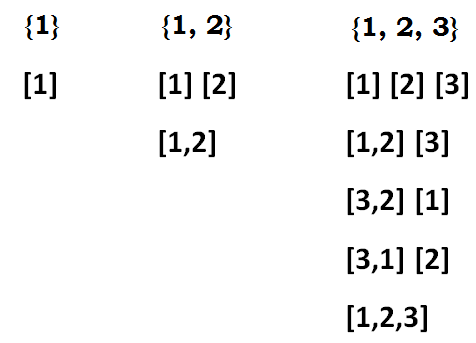
\includegraphics[scale=0.7]{ParticionesNegro.png}
	\end{center}
\end{figure}
Y si notamos la siguiente similitud entre la transición de uno a otro (ejemplo, transición de particionesDe2 a \\particionesDe3):\\
\begin{figure}[h]
	\begin{center}
	   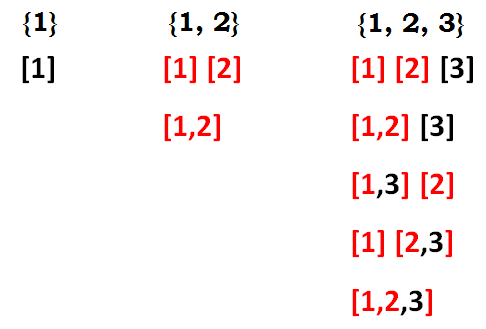
\includegraphics[scale=0.7]{ParticionesNegroRojo.png}
	\end{center}
\end{figure}\\
Veremos que las particionesDe3 son las particionesDe2 solo que agregando el 3  primero en un subconjunto aparte, y luego dentro de los subconjuntos de 2. Entonces:

\newpage
Para generar las particiones un conjunto de 3 elementos, a partir de las particiones de un conjunto de 2 elementos, hace 2 pasos:\\
\begin{enumerate}
\item Toma todas las de 2 elementos y le agrega un nuevo conjunto que solo contiene al 3 (en el gráfico, las 2 primeras particiones), ese nuevo grupo de particiones ya formará parte de las particiones finales de 3 elementos.\\
Esta cantidad de particiones añadidas cumple que \#particionesAñadidas = \#particionesTotalesDeN-1
\begin{figure}[h]
	\begin{center}
	   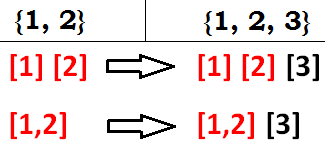
\includegraphics[scale=0.6]{explicacionPaso1.png}
	\end{center}
\end{figure}\\


\item Luego, vuelve a mirar las particiones de 1..2, y por cada una (llamemosle X) realizará lo siguiente:\\
\indent Añadirá una partición por cada subconjunto de X, y en cada una de ellas, agregará el valor de n (3 en este caso) a un subconjunto distinto para luego formar parte de las particiones finales buscadas.\\
\begin{figure}[h]
	\begin{center}
	   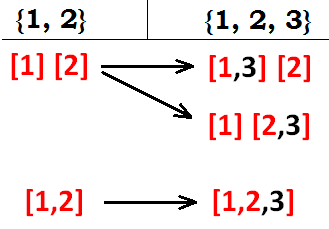
\includegraphics[scale=0.6]{explicacionPaso2.png}
	\end{center}
\end{figure}\\

\indent \textbf{\underline{Ej:}} Toma la partición \textbf{[1] [2]}:\\
\indent -Aplica el \textbf{3} al subconjunto \textbf{[1]}, quedando: \textbf{[1,3] [2]} que ya formará parte de las particiones finales.\\
\indent -Agrega a las particiones finales.\\
\indent -Revierte el 3 aplicado.\\
\indent -Luego aplica el \textbf{3} al subconjunto \textbf{[2]} de la misma partición, resultando en el conjunto: \textbf{[1] [2,3]}\\
\indent -Agrega a las particiones finales.

Y así se construyó la tercer y cuarta partición; repitiendo el procedimiento para la partición \textbf{[1,2]} se obtendrá la última partición de las 5.\\
\end{enumerate}
Esa es la \textbf{base} del algoritmo exacto utilizado para generar las particiones de un conjunto de números de tamaño n. Se deja guardada en el código la partición base, que es la única partición de un conjunto de 1 elemento, y para las demás se realiza el procedimiento mencionado n-1 veces, generando así las particiones de un conjunto de n elementos a partir de las de un conjunto de n-1.\\
Tiene una gran \textit{'pinta'} recursiva, pero decidimos hacerlo iterativo.\\

A continuación, el pseudocódigo del algoritmo (nuevamente, sin las podas):\\

\textbf{subConjunto} es un vector\textless Enteros\textgreater \\
\indent \textbf{Particion} es un vector\textless subConjunto\textgreater\\
\indent \textbf{PARTICIONES} es un vector\textless Particion\textgreater

\newpage
\underline{Recibe:}\\
-Un conjunto de particiones que esta vacío para que lo llene.\\
-El n
\begin{lstlisting}
getPartitionsOfN(n, PARTICIONES)

		PARTICIONES := {{1}}
	
		for i = 2 to n inclusive do
			lengthAnterior := PARTICIONES.length

			for j = 0 to lengthAnterior inclusive do
				jPartition := copyOf(PARTICIONES[j])

				PARTICIONES[j] U {i}			
					
				for p = 0 to jPartition.length hacer
					jPartition[p].push_back(i).
					PARTICIONES U {jPartition}.
					jPartition[p].pop_back();
				Fin Para
			
			end for
	
		end for

		devolver PARTICIONES;

end of getPartitionsOfN
\end{lstlisting}
---------------------------------------------------------------------------------------------------------------------------------------------------

\underline{\textbf{Las podas y estrategias:}}

\begin{enumerate}
\item \textbf{Poda de cantidad de conjuntos.}\\
Dado un n, la cantidad máxima de conjuntos que puede tener una particion de n es n. Pero las particiones de n tales que tienen mas de k conjuntos no nos interesan, ya que estamos en el problema de la k-PMP donde nos interesan las particiones que tengan a lo sumo k conjuntos.\\
Ejemplo utilizando las imágenes usadas para la explicación del algoritmo; en ese caso, n = 3. Si nuestro k (por ejemplo) es 2, ¿tendría sentido agregar la primer particion al conjunto de particiones final ([1][2][3])? No lo tendría puesto que por definición de una k-PMP no puede ser una solución del problema, y estaríamos generando particiones que luego analizariamos cuando ya sabemos de antemano que no son posibles.\\

\item \textbf{Poda de mejor peso encontrado hasta el momento.}\\
Esta poda se basa en que el peso de cualquier partición de n que tenga k o menos conjuntos es\textgreater = al peso de la solución óptima.
Dicho esto, si supieramos que alguna particion de n (y tamaño\textless = k) tiene peso X, entonces cuando estamos construyendo las particiones, si notamos que la particion que estamos construyendo ya sobrepasó ese límite (a pesar de que aún no tenga los n elementos), entonces no tiene sentido seguir construyendola ya que el peso intraparticion de los elementos ya aplicados lo superó y por lo tanto no es óptima. Si esto ocurre, se elimina esa partición de el conjunto de particiones credas hasta el momento.
Este valor X lo conseguimos mediante una \textit{cota inicial} que realizamos previo a la formación de las particiones de n, que será explicado en breve.\\

\item \textbf{Poda de actualización de mejor peso encontrado.}\\
En la poda recién explicada, se detallaba que dado un peso X calculado anteriormente, las particiones que se estén construyendo y alcanzaran dicho límite serían removidas. Pero ¿por qué no ir actualizando este límite si vamos encontrando particiones tales que ya tienen todos los nodos cargados y mejor peso que X?\\
Eso es lo que hace esta poda, si dada una partición U de n, tal que peso(U)\textless peso\_optimo\_parcial, entonces peso\_optimo\_parcial = peso(U). Esto permitirá que más particiones sean recortadas a futuro.\\
\textit{Aclaración:} Como se explicó, esta cota tiene utilidad recién cuando se encuentra una particion n. En nuestro algoritmo, no nos sirve mientras estamos construyendo las particiones de n-1, n-2,...,3,2 ya que necesitamos todos los nodos cargados para poder asegurar que encontramos un peso tal que peso\textless peso\_optimo\_parcial. Por ende somos conscientes que hasta la última iteración del for principal (pseudocódigo) no nos sirve, pero debido a que el peso de una partición actual en construcción ya lo calculamos para la poda anterior (poda número 2) realizar el checkeo y la asignación es O(1), así que no perdíamos nada por aplicarla.\\

\item \textbf{Estrategia previa para acotar el peso de la solución óptima.}\\
En esta estrategia, para obtener una cota superior de lo que puede llegar a pesar la solución óptima, decidimos ejecutar el algoritmo goloso antes del exacto (ejercicio 3 de este Trabajo Práctico) para que nos devuelva una configuración posible de los nodos (potencialmente óptima) y tomar su peso para usarlo como cota en la construcción de las particiones.\\
Si la cota devolviese la peor solución habría sido como si no hubiera existido, porque no hubiera acotado al problema.\\
\end{enumerate}

Dicho esto, a continuación el pseudocódigo \textit{con podas} de la parte del algoritmo que se encarga de la construcción de las particiones:\\

\begin{lstlisting}
getPartitionsOfN(pesos, n, k, PARTICIONES)

		PARTICIONES := {{1}}
	
		para i desde 2 hasta n inclusive hacer
			lengthAnterior := particiones.length

			para j desde 0 hasta lengthAnterior inclusive hacer		
				copy := copyOf(j-esima particion de PARTICIONES)

				Si la j-esima particion aun no tiene tamano igual a k
					agregar conjunto {i} a la j-esima particion			
				Sino
					Borrar la j-esima particion de PARTICIONES;
					j--;
					lengthAnterior--;
				Fin si
			
				Para p desde 0 hasta copy.length - 1 inclusive hacer
					copy[p].push_back(i);
					peso := peso(copy);
					
					Si peso < optimo_peso_parcial		
						Agregar copy a PARTICIONES
						Si i == n
							optimo_peso_parcial <- peso;					
						Fin Si
					Fin Si
					
					copy[p].pop_back();
					
				Fin Para
			
			Fin para
	
		Fin para

		return;

end of getPartitionsOfN
\end{lstlisting}
---------------------------------------------------------------------------------------------------------------------------------------------------
\newpage
\subsection{Análisis de la complejidad temporal}
Para la ejecución de la implementación del algoritmo (en C++), veremos el algoritmo en su peor caso, que es \textbf{sin ninguna cota aplicada}.\\
También, para los casos donde se realize el método push\_back() de la clase vector, si bien su costo es\\ \textbf{O(1) amortizado}, para simplificar el analisis de complejidad, se tomará como O(1).\\

Tenemos 3 ciclos a mirar.\\

\noindent \underline{El \textbf{primer ciclo for}}:\\
Itera un total de n-1 veces. Como es el for "padre", la complejidad temporal final será:

\textit{O(costo iteración 1) + O(costo iteración 2) + ... + O(costo iteración n-1)}. $\forall$\textit{n\textgreater =2}\\

\noindent Veamos el costo de cada iteración:

Se ejecuta solamente una asignación y \textbf{el segundo for}, por lo que la complejidad de cada iteración será igual a la complejidad de dicho segundo for en la misma iteración (la asignación es en O(1)). Veamoslá:\\

\noindent \underline{El \textbf{segundo ciclo for}}:\\
El for cicla tantas veces como la variable \textbf{lengthAnterior} indique.\\
Como dicha variable toma el tamaño de PARTICIONES, que al principio de cada iteración i del primer for contiene todas las particiones del conjunto \textit{\{1,2..i-1\}}, entonces la complejidad de dicho for será:

\textit{ O(\#particionesDeI-1 * costo de cada iteración del segundo for)}.

\noindent Veamos ahora el costo de cada iteración del segundo for.

\begin{enumerate}
\item Realizar el backup de una partición tiene costo \textit{O(n)} puesto que a lo sumo tiene a todos los nodos, es decir, n nodos.
\item Acceder a la j-esima posición de PARTICIONES y modificarlo agregandole un subConjunto tiene costo O(1).
\item Por último tenemos el costo del último for (tercer for), que itera los subConjuntos de la particion backupeada.
\end{enumerate}
Por lo que la complejidad temporal del segundo for en una iteración es:\\
\textit{O(n + costo del tercer for)}\\

\noindent \underline{El \textbf{tercer ciclo for}}:\\
Dada la j-esima partición backupeada en el segundo for, itera todos los subConjuntos. En el peor caso una partición puede tener n subConjuntos (1 nodo en cada uno), por lo que el costo es:\\
\textit{O(n * costo de cada iteración)}.

\noindent Donde el costo de cada iteración es:
\begin{enumerate}
\item Acceder a un conjunto y agregar un elemento: \textit{O(1)}.
\item Copiar la particion backupeada a PARTICIONES: \textit{O(n)}.
\item Acceder al último conjunto modificado y eliminar el elemento recién agregado: \textit{O(1)}.
\end{enumerate}
Costo final de cada iteración: \textit{O(n)}.\\

\noindent Por ende, el costo final \textbf{(de peor caso)} del tercer for es:

\textit{\textbf{O(n * n) = O($n^2$)}}\\ \\

Ahora, reemplazando la cota de complejidad conseguida del tercer for en el costo de \textbf{cada iteración del segundo for} nos queda:

\textbf{\textit{O(n + costo del tercer for) = O(n + $n^2$) = O($n^2$)}}

\noindent Volviendo a la complejidad del segundo for en una iteración i del primer for, teníamos:

\textit{O(\#particionesDeI-1 * costo de c/iteración del segundo for)}. = \textbf{\textit{O(\#particionesDeI-1 * $n^2$)}}

\newpage
Volviendo a la complejidad del primer for, teníamos que el costo total del algoritmo era:

\textit{O(costo iteración 1) + O(costo iteración 2) + ... + O(costo iteración n-1)}. $\forall$\textit{n\textgreater =2}\\
Donde \textit{costo iteración i} es el costo del segundo for en la iteración i del primer for.\\

Reemplazando lo conseguido del análisis del segundo for, el costo total del algoritmo es:

\textbf{\textit{O(\#particionesDe1 * $n^2$)) + O(\#particionesDe2 * $n^2$) + ... + O(\#particionesDeN-1 * $n^2$)}}.\\



\underline{Analizando la cantidad de particiones posibles distintas de un conjunto de N elementos.}\\
Los \textbf{\textit{Números de Bell}} (http://en.wikipedia.org/wiki/Bell\_number) son los números que indican la cantidad de particiones distintas posibles de un conjunto dado. Los mismos fueron presentados por \textit{Eric Temple Bell} y se definen bajo la siguiente fórmula \textbf{recursiva}:\\

INSERTE LATEX AQUI DE LA FORMULA DE BELL.\\

Se conocen distintas cotas superiores de estos números (http://en.wikipedia.org/wiki/Bell\_number\#Growth\_rate), y la que vamos a usar es la establecida por \textit{Berend. y Tassa. (Improved Bounds on Bell Numbers and on Moments of Sums of Random Variables)}, la cual acota superiormente al termino Bn de los números de Bell por la siguiente relacion:\\

INSERTE LATEX AQUI DE LA COTA.\\ \\


\noindent Luego, como la cantidad de particiones de un conjunto es estrictamente creciente en el tamaño del mismo, volviendo a donde habíamos quedado con respecto a la complejidad total del algoritmo:

\noindent \textit{O(\#particionesDe1 * $n^2$)) + O(\#particionesDe2 * $n^2$) + ... + O(\#particionesDeN-1 * $n^2$)} $\in$

\noindent \textit{O((n-1) * (\#particionesDeN-1 * $n^2$))} $\in$ 

\noindent \textit{O($n^3$ * \#particionesDeN-1)} $\in$ (Usando la cota mencionada)

\noindent \textit{O($n^3$ * $((n-1)/ln(n-1+1))^n$)}.\\

Finalmente, removiendo constantes:

\textbf{\textit{O($n^3$ * $(n/ln(n))^n$)}} que es una cota de la complejidad temporal final del algoritmo\\ \\ \\

\underline{\textbf{Análisis con las podas aplicadas}}

Las podas aplicadas al algoritmo en sí (dejando de lado la ejecución previa del algoritmo goloso) son las 3 primeras mencionadas anteriormente.

Para la \textbf{primer poda}, se agregó un if que en cada iteración del segundo for consulta por el tamaño actual de la partición para evitar revisar particiones de más de k conjuntos.\\
Dado que el método \textit{.size()} de vector es en \textit{O(1)}, la guarda del if se ejecuta en tiempo constante.\\
Si se ingresa por el if la ejecución continúa su flujo normal, de lo contrario, se hacen 2 operaciones básicas y un borrado, el cual en peor caso tiene costo \textit{O(n)}, por lo que no modifica la complejidad ya que previo a eso se había invertido O(n) en copiar la instancia, y porque el mayor costo lo tiene el tercer for con \textit{O($n^2$)}.\\
Eliminar dicha instancia evita que se siga ramificando apartir de ella un subárbol de desiciones que crece exponencialmente y que no tiene sentido revisar.\\
También, evitando generar esas particiones no solo ganamos temporalmente, sino también (en la práctica) en la espacialmente.

Para la \textbf{segunda poda}, se hace la medición del peso de la partición durante el tercer for antes de agregarla al conjunto de particiones final. Esta validación no se hace cuando se agrega un conjunto nuevo aparte (antes del tercer for) ya que agregar un conjunto con un solo elemento no modifica el peso de las aristas intrapartición.\\
Calcular el peso de la partición tiene costo \textit{O($n^2$)}, por lo cual, teóricamente estamos perdiendo complejidad, ya que cada iteración del tercer for ya no cuesta \textit{O(n)}, sino \textit{O($n^2$ + n) = O($n^2$)}, pero en la práctica favoreció de una manera muy positiva cuando trabaja en conjunción con la cota superior dada por el algoritmo goloso.

Finalmente para la \textbf{tercer poda}, se hace la actualización del peso\_optimo\_parcial. Esto se realiza mediante un if con una guarda que se ejecuta en \textit{O(1)}, al igual que el cuerpo del mismo.\\
Esto es así ya que el peso de la partición lo teníamos calculado y guardado cuando lo utilizamos en la segunda poda.\\

\noindent En conclusión, las podas no empeoraron la complejidad del algoritmo, a excepción de la poda numéro 2, que si bien, por el análisis teórico transforma \textit{O(n)} en \textit{O($n^2$)}, trabajando conjuntamente con el algoritmo goloso ejecutado previamente, es la poda que más eficiencia nos provió.\\
El caso en el que esta poda no tenga efecto positivo sobre el algoritmo y finalmente termine siendo una contra, sería el caso en el que el algoritmo goloso devuelva la peor partición posible de los nodos, lo cual tiene una ínfima posibilidad de ocurrir.\\

\noindent \textbf{\textit{Nota: }} En cuanto al algoritmo goloso no se hace un análisis del mismo puesto que eso ya fue hecho en el ejercicio 3 de este trabajo práctico.\\Además, este presenta una complejidad polinomial, la cual es despreciable en comparación con las escalas de complejidad que ronda el algoritmo exacto en sí.




  
\newpage
\subsection{Experimentación}
Para la experimentacion, se realizaron distintos escenarios de test. Cada escenario contiene valores que son producto de distintas tomas de datos del algoritmo en ejecución.

Como es sabido, la computadora en la que se realizaron las mediciones, no está atentiendo nuestro proceso únicamente. Es por eso, que realizar una única medición de cada instancia no nos asegura fidelidad.\\
\indent Para aminorizar esta falencia, se repitió cada instancia de cada caso de test de cada escenario, un total de 10 veces, y se tomó el mejor tiempo.\\
Notar que tomar el mejor tiempo (en lugar del promedio) no es una mala desición, ya que entre 2 mediciones de tiempos distintas, t1 y t2, si t1\textless t2, eso nos asegura que en t1 el procesador estuvo más focalizado en nuestro proceso, y por ende, es una medición más fiel del mismo.

Para realizar las mediciónes, se realizó un generador de instancias aleatorias, que dada una cantidad de nodos (n), una cantidad de aristas (m) y un entero (k), genera de forma aleatoria m aristas, tomando para cada una, 2 nodos de n, que no tengan ya una arista entre ellos.

También, para el escenario de un k dado, no se hicieron pruebas donde ocurra que k\textgreater =n, ya que la respuesta de estos casos es trivial, (que cada nodo podría ir en un conjunto distinto). Hacer las mediciones de un caso trivial no tiene mucho sentido, por lo que en todas las mediciones, siempre vale que k\textless n.

En todos los casos se midieron grafos de n nodos, que tengan una densidad de aristas del 25\%, 50\%, 75\% y 100\%.

Los valores de k elegidos fueron 3, 5, 8 y 13, que siguen la serie de \textit{Fibonacci} para una variación más uniforme.\\

\underline{\textbf{Los escenarios:}}
\textbf{\textit{ESCENARIO CON K = 3:}}
	\begin{figure}[h]
		\begin{center}
		   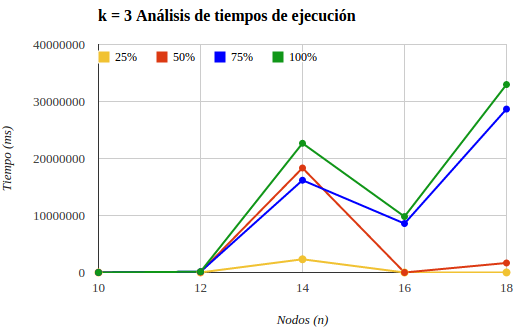
\includegraphics[scale=0.70]{graficos/k3.png}
		\end{center}
	\end{figure}\\
	\begin{figure}[h]
		\begin{center}
		   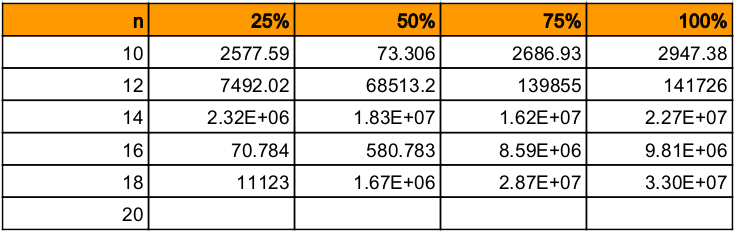
\includegraphics[scale=0.50]{graficos/tablak3.png}
		\end{center}
	\end{figure}\\

	
\newpage	
\textbf{\textit{ESCENARIO CON K = 5:}}
	\begin{figure}[h]
		\begin{center}
		   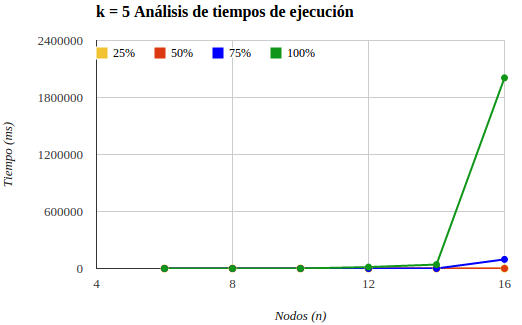
\includegraphics[scale=0.70]{graficos/k5.png}
		\end{center}
	\end{figure}\\
	\begin{figure}[h]
		\begin{center}
		   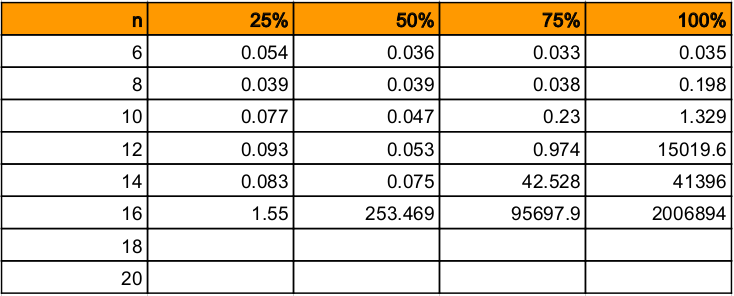
\includegraphics[scale=0.50]{graficos/tablak5.png}
		\end{center}
	\end{figure}\\
\newpage
\textbf{\textit{ESCENARIO CON K = 8:}}
	\begin{figure}[h]
		\begin{center}
		   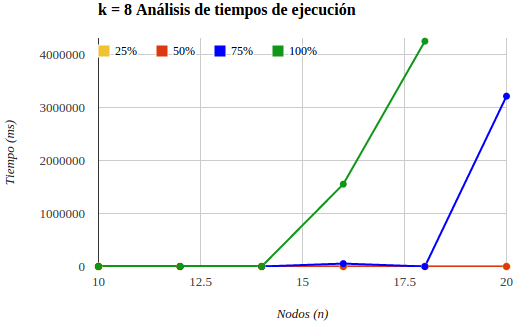
\includegraphics[scale=0.70]{graficos/k8.png}
		\end{center}
	\end{figure}\\
	\begin{figure}[h]
		\begin{center}
		   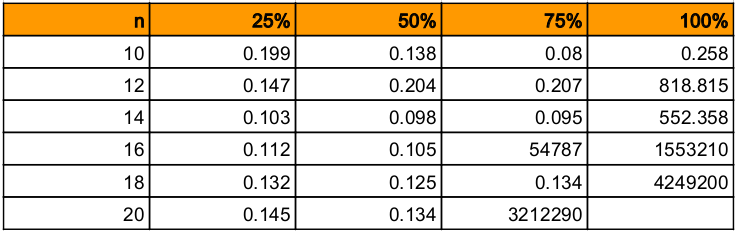
\includegraphics[scale=0.50]{graficos/tablak8.png}
		\end{center}
	\end{figure}\\
	
\newpage
\textbf{\textit{ESCENARIO CON K = 13:}}
	\begin{figure}[h]
		\begin{center}
		   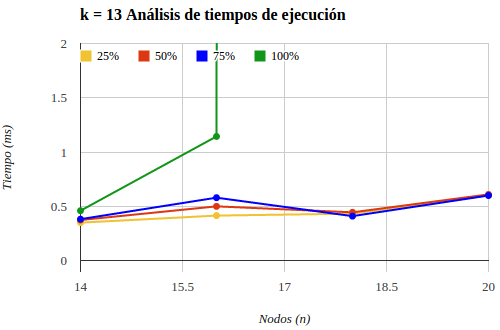
\includegraphics[scale=0.50]{graficos/k13ConZoom.png}
		\end{center}
	\end{figure}\\
\indent Si le alejamos un poco el zoom...
	\begin{figure}[h]
		\begin{center}
		   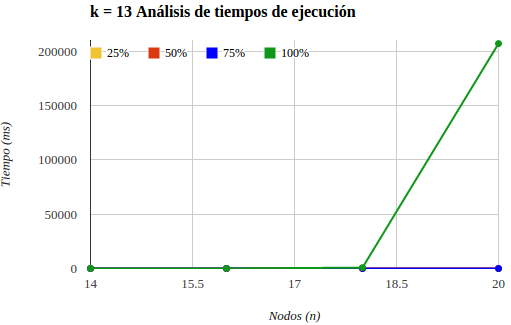
\includegraphics[scale=0.50]{graficos/k13SinZoom.png}
		\end{center}
	\end{figure}
	\begin{figure}[h]
		\begin{center}
		   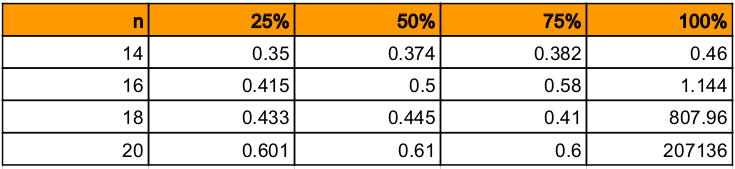
\includegraphics[scale=0.50]{graficos/tablak13.png}
		\end{center}
	\end{figure}\\

\end{document}